\section*{Übung 10}
\subsection*{Aufgabe 1}
\subsubsection*{Lösungsidee}
Es wird eine Prozedur erstellt, basierend auf der vorgeschlagenen Lösungsidee. Um die Größe des Arrays festlegen zu können wird die Anzahl der Nodes im Baum mithilfe von CountNodes ermittelt. Nachdem das Array initialisiert wurde und alle Nodes des Baumes in das Array eingefügt sind, werden die Mittelpositionen berechnet. Mit den berechneten Werten wird bestimmt welche Elemente des Arrays eingefügt werden. Elemente die bereits in den Baum gespeichert wurden, werden im Array auf NIL gesetzt. Alle fehlenden Elemente werden danach eingefügt.
\newline

\lstinputlisting[language=Pascal] {../balancedtree.pas}
\begin{figure}[H]
	\centering
	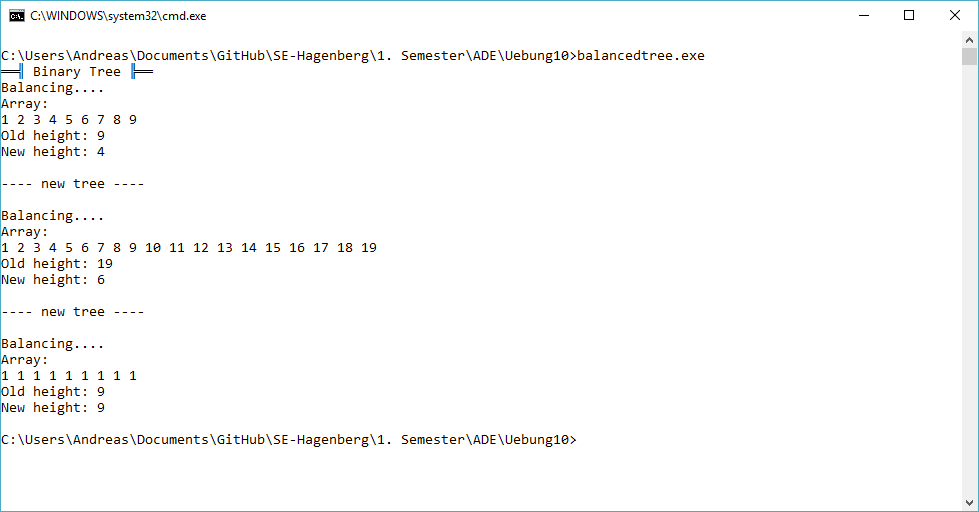
\includegraphics[scale=0.65]{./pictures/balancedtree.png}
	\caption{Testfälle}
	\label{fig: BalancedTree}
\end{figure}

\subsection*{Testfälle}
Die Testfälle zeigen drei verschiedene Bäume mit unterschiedlicher Länge und Werten. Anhand des dritten Baumes wird ersichtlich das bei gleichen Werten die Höhe des Baumes nach dem Balancieren die gleiche ist wie davor.

\subsection*{Zusatzfrage}
Da bei diesem Baum nicht extra spezifiziert wurde was mit gleichen Werten geschehen soll wird immer nur in eine Richtung eingefügt, die Zahl ist schließlich nicht größer als die Wurzel oder der jeweilige Knoten. Damit ergibt sich selbst nach dem ausführen des Algorithmus immer noch dieselbe Höhe.
\newpage


\subsection*{Aufgabe 2}
Anhand dieser Funktion und mit der nachfolgenden Tabelle soll eine Formel erstellt werden mit der die Laufzeit der Funktion berechnet werden kann.\newline

\lstinputlisting[language=Pascal] {../code_2.pas}

\begin{center}
\begin{tabular}{|c|c|c|c|c|}
\hline
Operation               & Ausführungszeit 	\\ \hline 
Wertzuweisung           & 1		            \\ \hline 
Vergleich               & 1 		        \\ \hline 
Indizierung             & 0,5		        \\ \hline 
Addition, Subtraktion 	& 0,5 		        \\ \hline 
Multiplikation 	        & 3 		        \\ \hline 
Prozeduraufruf 	        & 16 + 2 * Anzahl der Parameter		\\ \hline 
\end{tabular}
\captionof{table}{Laufzeiten}
\end{center}
\raggedright
Damit ergibt sich folgende Formel: $26 * length(input) + 1,5 * Count1(input) + 22 $
\newline
\newline
Length(input) bestimmt die Länge bestimmt die Länge der Eingabe, Count1 steht für die Anzahl der vorkommenden '1'.
\newline
\newline
Für die Binärzahlen 100100, 100001, 110100, 1111, 0000, 1 und 0 ergeben sich folgende Laufzeiten:

\begin{center}
\begin{tabular}{|c|c|c|c|c|}
\hline
Input    & Laufzeitlänge \\ \hline 
100100   & 181 	\\ \hline 
100001   & 181	\\ \hline 
110100   & 182,5 	\\ \hline 
1111     & 132	\\ \hline 
0000	 & 126	\\ \hline 
1 	     & 49,5	\\ \hline 
0 	     & 48	\\ \hline 
\end{tabular}
\captionof{table}{Laufzeiten Formel}
\end{center}
\raggedright

\subsubsection*{Vereinfachung}
Unter der Annahme das die Anzahl der vorkommenden '1' etwa der Anzahl der vorkommenden '0' entspricht, kann die Formel vereinfacht werden: $26,75 * length(input) + 22 $ 
\newline
\newline
Damit ergeben sich bei den vorgegebenen Längen folgende Laufzeiten:

\begin{center}
\begin{tabular}{|c|c|c|c|c|}
\hline
Länge    & Laufzeitlänge \\ \hline 
1     & 48,75 	\\ \hline 
2     & 75,5 	\\ \hline 
3     & 102,25 	\\ \hline 
4     & 129 	\\ \hline 
5     & 155,75 	\\ \hline 
6     & 182,5 	\\ \hline 
7     & 209,25 	\\ \hline 
8     & 236 	    \\ \hline 
9     & 262,75 	\\ \hline 
10    & 289,5 	\\ \hline 
11    & 316,25 	\\ \hline 
12    & 343 	\\ \hline 
13    & 369,75 	\\ \hline 
14    & 396,5 	\\ \hline 
15    & 423,25 	\\ \hline 
16    & 450 	\\ \hline 
17    & 476.75 	\\ \hline 
18    & 503.5 	\\ \hline 
19    & 530.25 	\\ \hline 
20    & 557	    \\ \hline 
50    & 1.359,5	\\ \hline 
100   & 2697	    \\ \hline 
200	  & 5.372	\\ \hline 

\end{tabular}
\captionof{table}{Laufzeiten vereinfachte Formel}
\end{center}

\subsubsection*{Asymptotische Laufzeitkomplexität}
Da die Formel eine lineare Funktion beschreibt(konstante Steigung), ist die asymptotische Laufzeitkomplexität linear. In der Tabelle sieht man das bei einer Änderung der Wortlänge um 1 jedes mal ein konstanter Wert hinzugefügt wird.

\newpage
\subsection*{Aufgabe 3}
Es wird wieder eine Tabelle mit nachfolgendem Code und mit der oben erwähnten Tabelle Laufzeiten. Dabei ergibt sich folgende Formel: $2,5 * length(input) + 23 * Count1(input) + 22,5 * length(input) - count1(input) + 39$
\newline
\newline

\lstinputlisting[language=Pascal] {../code_3.pas}

Für die Binärzahlen 100100, 100001, 110100, 1111, 0000, 1 und 0 ergeben sich folgende Laufzeiten:

\begin{center}
\begin{tabular}{|c|c|c|c|c|}
\hline
Input    & Laufzeitlänge \\ \hline 
100100   & 190 	\\ \hline 
100001   & 190	\\ \hline 
110100   & 190,5 	\\ \hline 
1111     & 141	\\ \hline 
0000	 & 139	\\ \hline 
1 	     & 64,5	\\ \hline 
0 	     & 64	\\ \hline 
\end{tabular}
\captionof{table}{Laufzeiten Formel}
\end{center}
\raggedright

\subsubsection*{Vereinfachung}
Unter der Annahme das die Anzahl der vorkommenden '1' etwa der Anzahl der vorkommenden '0' entspricht, kann die Formel vereinfacht werden: $48 * length(input) + 39$
\newpage
Damit ergeben sich bei den vorgegebenen Längen folgende Laufzeiten:

\begin{center}
\begin{tabular}{|c|c|c|c|c|}
\hline
Länge    & Laufzeitlänge \\ \hline 
1     & 87 	\\ \hline 
2     & 135 	\\ \hline 
3     & 183 	\\ \hline 
4     & 231 	\\ \hline 
5     & 279 	\\ \hline 
6     & 327 	\\ \hline 
7     & 375 	\\ \hline 
8     & 423 	\\ \hline 
9     & 471 	\\ \hline 
10    & 519 	\\ \hline 
11    & 567 	\\ \hline 
12    & 615 	\\ \hline 
13    & 663 	\\ \hline 
14    & 711 	\\ \hline 
15    & 759 	\\ \hline 
16    & 807 	\\ \hline 
17    & 855 	\\ \hline 
18    & 903 	\\ \hline 
19    & 951 	\\ \hline 
20    & 999	    \\ \hline 
50    & 2.439	\\ \hline 
100   & 4.839	\\ \hline 
200	  & 9.639	\\ \hline 

\end{tabular}
\captionof{table}{Laufzeiten vereinfachte Formel}
\end{center}

\raggedright

Die asymptotische Laufzeitkomplexität ist wieder linear. Man kann beobachten das der rekursive Algorithmus eine höhere Laufzeit hat als der iterative Algorithmus. Das liegt vor allem daran das bei der rekursiven Lösung immer wieder ein Funktionsaufruf stattfindet.